%\RequirePackage[l2tabu, orthodox]{nag}

\documentclass[11pt,oneside]{report}
\usepackage[a4paper, margin=1.5in]{geometry}
%\usepackage{fullpage}
\usepackage{url}
\usepackage{tabularx}
\usepackage{graphicx}
\usepackage{harvard}
\usepackage{mathtools}
\usepackage{parskip}
\usepackage{subcaption}
\usepackage{bashful}
\usepackage{microtype}
\usepackage{float}
\usepackage{hyperref}
\usepackage{fancyhdr}
\usepackage{gensymb}
\usepackage{multirow}
\usepackage{listings}
\usepackage{color}
\usepackage[font={small,it}]{caption}
\usepackage[toc,page]{appendix}


\usepackage{inconsolata}

\definecolor{pblue}{rgb}{0.13,0.13,1}
\definecolor{pgreen}{rgb}{0,0.5,0}
\definecolor{pred}{rgb}{0.9,0,0}
\definecolor{pgrey}{rgb}{0.46,0.45,0.48}
\lstset{
  numbers=left,  
  language=Java,
  showspaces=false,
  frame=leftline,
  showtabs=false,
  breaklines=true,
  showstringspaces=false,
  breakatwhitespace=true,
  commentstyle=\color{pgreen},
  keywordstyle=\color{pblue},
  stringstyle=\color{pred},
  basicstyle=\ttfamily\scriptsize,
  moredelim=[il][\textcolor{pgrey}]{!!},
  moredelim=[is][\textcolor{pgrey}]{\%\%}{\%\%},
  captionpos=b,
  inputpath=./src
}

\pagestyle{fancy}
\fancyhf{}
\rhead{\thepage}
\lhead{\leftmark}

\cfoot{}

\citationmode{abbr}
\renewcommand{\baselinestretch}{1.5}
\newcommand\code[1]{\texttt{#1}}
\newcommand{\varusecase}{\textbf{Use case}}
\newcommand{\vardescription}{Description}
\newcommand{\varactor}{Actor}
\newcommand{\varentry}{Entry Condition}
\newcommand{\varflow}{Flow of Events}
\newcommand{\varaltflow}{Alternative Flow}
\newcommand{\varexit}{Exit Condition}

%\renewcommand{\familydefault}{\sfdefault}


\graphicspath{{images/}}

\title{An Open Source Computer Vision Framework for Leap Motion}
\author{Daniel Hamilton 10026535,\\Computer Science,\\University of the West of England.}
	
\bash
texcount -merge -sum -1 -opt=TCOpt.txt report.tex
\END

\begin{document}
	\maketitle
	
	\begin{abstract}
	
	\end{abstract}	
	
	\renewcommand{\abstractname}{Acknowledgements}
	\begin{abstract}
	
	\end{abstract}
	
	\tableofcontents
	\listoffigures
	\listoftables
	\renewcommand{\lstlistlistingname}{List of Listings}
	\lstlistoflistings

	Word Count: \bashStdout.

	%----------------------------------------- Chapter 1 -----------------------------------------%
	\chapter{Introduction}\label{chap:introduction}
		\section{Computer Vision: An Intellectual Frontier}
			\subsection{What is Computer Vision?}		
				
				It is very hard for humans to know what their own biological vision really entails, and how difficult it is to reproduce on a computer.
				Information from the eyes is divided into multiple channels, each streaming different kinds of information to the brain.
				The brain then subconsciously groups and identifies the parts of the image to examine along with what parts to suppress.
				The way in which biological vision works is still largely unknown which makes it hard to emulate on computers \cite[p. xi]{book:multiViewGeo}.				
				Computer vision systems are still relatively naive, all they "see" is a grid of numbers.%from def:cv
				
				%By default there is no built in pattern recognition, or what some might call, intelligence.
				
				Computer vision is a vast field and hard to define.
				For the purpose of this report it will be defined as:
	
				\begin{quote}
					``\textit{The transformation of data from a still or video camera into either a decision or a new representation.
						All transformations are done for achieving some particular goal.}'' \cite[p. 2]{definition:cv}
				\end{quote}
				
				Even though computer vision in terms of comparison to biological vision, still remains an unsolved problem, there have still been many excellent achievements in the field to date.
			\subsection{Uses of Computer Vision}
				One of the most prominent uses of computer vision currently, is in driver less cars.
				In recent years, they have reached a level of sophistication at which they are being approved by governments to be used on public highways \cite{web:driverlessCars}.
				Complex and expensive equipment with the capability to analyse a three-dimensional scene in real-time is usually required to achieve this.
				%Add the http://velodynelidar.com/lidar/hdlproducts/hdl64e.aspx here, try and find a price to reference "expensive" maybe mention google explicitely.
				Computer vision is also used on production lines.
				\citeasnoun{journal:salmon} set out to try and classify salmon fillets, to see if it was possible to determine whether a salmon fillet had been processed using enzymes. %maybe expand on what they actually did experementally here.
				However, computer vision isn't only available to big companies with large amounts of money to spend on research.
				\begin{quote}
				``\textit{Computer vision is a rapidly growing field, partly as a result of both cheaper and more capable cameras, partly because of affordable processing power, and partly because vision algorithms are starting to mature.}''\cite[p. ix]{definition:cv}
				\end{quote}
				One such device that has been made available is the Kinect by Microsoft.
				The computer vision society found that the capabilities of the Kinect could be extended beyond its intentional use for gaming, and at a much lower cost than traditional three dimensional cameras.
				It has been used in areas such as human activity analysis, where it is able to estimate details about the pose of the human subject in its field of vision \cite{kinect:1}.
				It has also been used to for real time odometry whilst attached to a quadcopter, enabling the production of a three dimensional mapping of a physical space \cite{kinect:2}.
				%The line below is dependant on a reference
				A hacking culture has enabled this type of exploitation of technology to take place and is spurring the creators of these technologies to make them more open.
				
		\section{The Leap Motion Controller}
			\subsection{What is the Leap Motion?}
				%cite leapmotion https://developer.leapmotion.com/articles/intro-to-motion-control
				The Leap Motion Controller is a device aimed at providing a Natural User Interface through hand gestures.
				It is made up of two infra red cameras both with a fisheye lense, set up stereoscopically.
				Figure~\ref{fig:leapIR} shows an infra red image of the leap motion cameras and infra red lighting.
				\begin{figure}[!ht]
				\begin{center}
					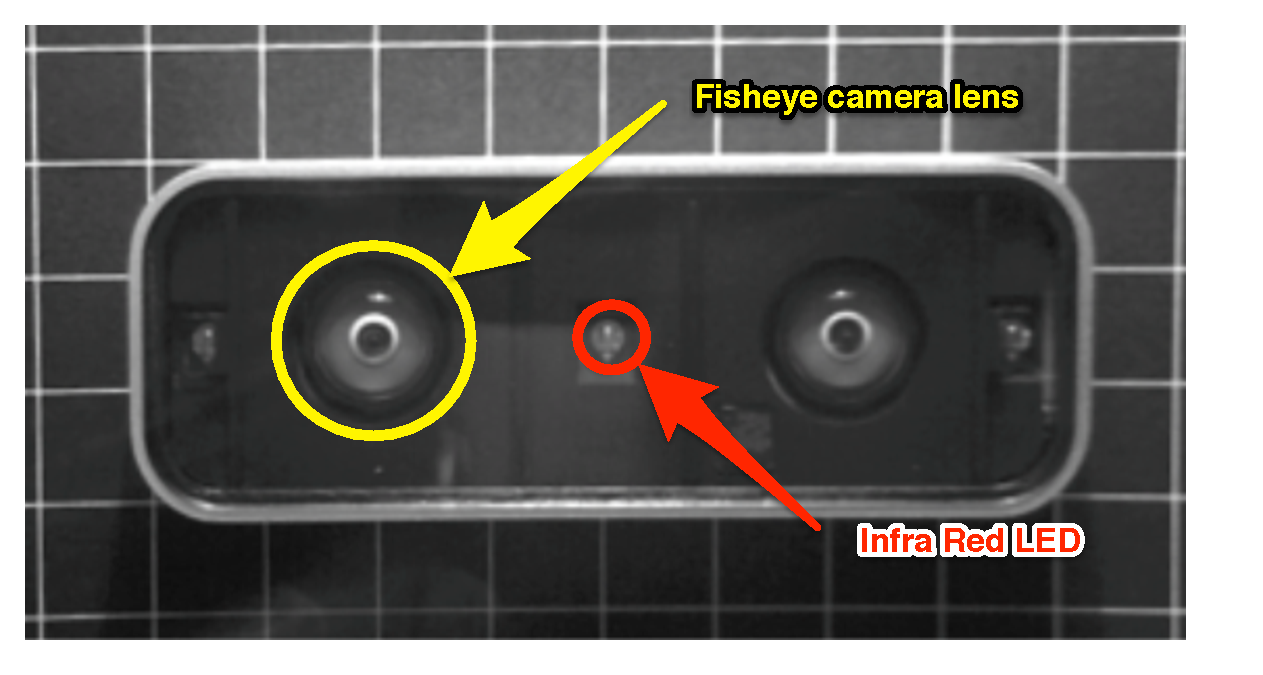
\includegraphics[width=\textwidth]{leap_ir.pdf}
					\caption{Infra Red Image Showing Leap Motion Internals\protect {\label{fig:leapIR}}}
				\end{center}
				\end{figure}
				It provides functionality out of the box that allows a developer to track movements and gestures made by a hand \cite{web:leapGestures}.
				%Don't really need the price...
				Leap motion have recently released a new version of their SDK, allowing access to more elements of their Leap Motion Controller. 
				Namely, images from the two cameras. 
				This could possibly be exploited in computer vision. %define disparity
				The  SDK is closed source, therefore it is not known the current methods by which hands and gestures are classified \cite[p. 217]{journal:leapEvaluation}.
				With the access to the images it allows exploration of other, custom methods for object classification and tracking.
				The SDK is for C++, C\#, Objective-C, Java, Python and Javascript.
				It works on Microsoft Windows, Mac OS X and a variety of Linux systems.
				There are currently iOS and Android libraries that are available through request.
				It is therefore a truly multi platform device.
				
				The leap motion is an extremely accessible device and it can be purchased for a price in the range of \pounds55\footnote{\url{http://www.amazon.co.uk/Leap-Motion-Controller-Interacts-Airspace/dp/B00C66Z9ZC}}.
				It is small in size with dimensions 80mm $\times$ 30mm $\times$ 11.25mm.
				
				
				

			\subsection{Uses in Computer Vision}
				The Leap Motion Controller has already been used in many innovative ways.
				An example of this is its use in recognising Australian and Arabic sign language \cite{journal:leapSignLanguage,journal:leapSignLanguage2}.
				However, these solutions only make use of the default detection system in the SDK.
				The default detection system is advanced and accurate enough to detect hand movements to this scale but raw image access is required to detect objects other than hands.
				As stated previously, image access has now been given, and so a whole new future of possibilities have been opened.
				Having access to the images allows for their use in computer vision.
				In turn this means that such an accessible and small device can be used in a variety of new ways.
				By creating an open source computer vision framework for the leap motion, it might become of use in the field of robotics.
				For example, it's size would make it suitable to attach to a robot as a rudimentary depth sensing system for collision avoidance.
				
				%need to talk about its use in areas such as robotic arms to pick up things for packaging etc.
			
		\section{Current State-of-the-Art}
		
			\subsection{OpenCV}
				OpenCV is an extensive Computer Vision framework that has grown out of a research project, initially run by Intel.
				Universities were seen to be sharing internal computer vision infrastructures between students, and so OpenCV was conceived to make this type of infrastructure universally available.
				Its first alpha release was made available in January 1999.
				One of its goals is to provide a simple-to-use computer vision infrastructure that helps people build fairly sophisticated vision applications quickly \cite[p. 1]{definition:cv}.	
				By making computer vision more accessible, Intel were increasing the need for faster processors, in turn generating themselves more income \cite{definition:cv}.
				
				Computer vision is computationally expensive.
				However, many scenarios that use computer vision, need to happen in real time.
				OpenCV was designed for computational efficiency with a strong focus on real-time applications.
				Early on in its life, Intel had pushed for the requirement of more power from CPUs.
				Then in 2010 GPU acceleration was added to OpenCV.
				It has been developed so that adoption from the CPU library to the GPU library is easy, so that developers do not require any training.
				\citeasnoun{journal:nvidia} have shown this extension has sped up algorithms up to four times on a GPU than a CPU.
				
				While the original library is written in C/C++, it has also been wrapped to work on iOS and Java/Android platforms.
				With smartphone processors often improving in each new release, as well as built in cameras, the demand for computer vision applications is increasing.
				Currently, devices are capable of stitching together several photographs into a high resolution panoramic image in real time.
				As well as having the capability of using facial recognition to unlock the device \cite{journal:face}.
				
				Since its first release the library has become well established in the Computer Vision field.
				A simple search with the term ``\textit{OpenCV}'' on google scholar, returns about 38,700 results.
				With the \citeasnoun{definition:cv} book itself cited by 3409 others.
				
				OpenCV is licensed under the BSD open source licence.
				Meaning it is open and free.
				The code can be embedded in other applications for research or for profit and there is no obligation that the created applications code needs to be open or free.
		\section{The Problem}
				Currently, there is no simple solution that allows a developer to simply plug in a leap motion and start developing for computer vision.
				While a computer vision expert might be able to start programming straight away, a non-expert would have to learn a large amount before they start to see any results.	
				
		\section{The Purpose}
				The main purpose is to try and expand the areas on the leap motion can be developed with.
				To try and find out whether it is feasible to say that a leap motion can be used for computer vision in a simple way.
				For example, to detect objects other than hands and tools with only a few function calls.
				
				This might start a new interest in computer vision.
				Allowing these non-experts that might have thought it too difficult before, to experiment in a new and easy way.
				There is a large community of interest in the leap motion forums, with many different projects using the current SDK.
				It might be assumed from the mere interest on threads that contain any form of reference to computer vision, that carrying out research on this will be a useful piece of work.
		\section{Hypothesis}
				It is possible to use the leap motion in the field of computer vision, so that application developers can exploit the technology in different ways as to what was originally intended.	
				This ability can then be structured into a framework, so that the effort application developers have to put in to use the leap motion as a solution, is low, making it an option to consider in new projects.	
		\section{Solution Approach}	
			It is envisaged that the framework will be made possible by taking advantage of functionality of the OpenCV library.
			Then exploiting the new image functionality of the leap motion SDK as mentioned earlier.
			The next few sections will outline the processes that will be followed to keep the project within a realistic scope and enable its completion.
					
		\section{Aim and Objectives} 
		This section outlines what the scope of the project is to be.
		The success of this project will be calculated based on the completion of each of the aim and objectives.
		\subsection{Aim}
		\begin{itemize}
			\item To develop an open source Computer Vision framework usable by the leap motion community.
			\item Enable the leap motion to recognise simple three dimensional shapes.
		\end{itemize}
		\subsection{Objectives} 
		\begin{itemize}
			\item Research methods for stereoscopic image object recognition.
			\item Research stereoscopic image processing methods.
			\item Design and develop a framework that allows the leap motion to be used for computer vision.
			\item Evaluate the accuracy of object recognition.
			\item Release an open source framework.
			\item Produce a report that communicates my findings
		\end{itemize}
			
		\section{Development Methodology}
					There are lots of development methodologies available for consideration.
					It is important to follow a development methodology to
					\begin{itemize}
						\item Divide a large problem into easy to understand tasks.
						\item Sharpen focus.
						\item Improve time estimates.
						\item Provide progress visibility.
						\item Provide better structure.
						\item Lead to better coding and documentation.
					\end{itemize}\cite{book:dawson}.
					
					As this is not a team based project, methodologies such as SCRUM will not be considered.
					Neither will a conventional waterfall model be considered, as this project has a relatively high uncertainty in user requirements.
					Many requirements will be explored throughout the development process.
					Therefore an iterative approach will be followed.
					With the first iteration being an example of a throw away prototype so as to explore technical uncertainties and ascertain initial requirements and scope estimate.
					The later iterations will then follow more of an evolutionary prototype approach.
					Where a large upfront requirements analysis and design takes place in the first of the evolutionary prototypes.
					This will be based on knowledge gained in the first iteration but not so much the implementation from the first iteration.
					It will aim to have a good base structure for the rest of the iterations to be evolved from.
					With tweaks to requirements happening in later iterations based on the evaluation of the previous implementation.
					Figure \ref{fig:iterative} gives a visual representation of the iterative approach.
					\begin{figure}[!h]
						\begin{center}
					
    						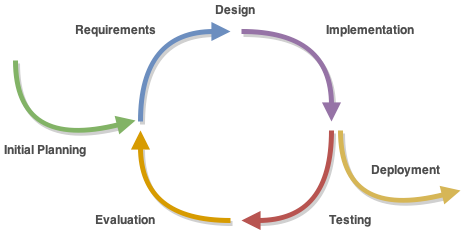
\includegraphics[width=\textwidth]{iterative_development}
    						\caption{Overview of an iterative development methodology {\label{fig:iterative}}}
    					\end{center}
					\end{figure}
			\subsection{Planned Iterations}
					During each iteration a test bench application will be developed that will make use of the framework.
					The development of this prototype will depend upon what level to which the framework is completed.
					Throughout each iteration sufficient unit tests will be implemented based on the requirements.
					Below is an outline of what work is aimed to be completed in each iteration.
					The work breaks down three discrete sections
					\begin{enumerate}
						\item Image processing
						\item Object detection
						\item Classification
					\end{enumerate}
					Each section in the order of the list, is dependant on the previous work being completed.	
					Therefore each iteration will aim to solve the work break down in order.
					Each iteration will be fully documented in chapter~\ref{chap:des&imp}.
					\subsubsection{Iteration 1}
					The first iteration will be an initial throwaway prototype.
					It will be used to explore the technologies that are going to be used in the project.
					Mainly to find out how the extensive OpenCV library works, and how well it will interface with the leap motion SDK.
					Image processing and stereo image processing will be explored here.
					Once completed it will allow better requirements to be established for the framework.
					\subsubsection{Iteration 2}
					The second iteration will be the first of an evolutionary prototype.
					It will better expand on the knowledge that will be obtained in iteration 1.
					It will implement the foundation upon which the whole framework will be based.
					The initial requirements will be established here so that a high level design can be accomplished.
					It is hoped that most of the image processing and stereo image processing functionality will be implemented in this stage.
					Providing a solid integration of OpenCV and the leap motion SDK.
					\subsubsection{Iteration 3}
					The third iteration will be the second stage of an evolutionary prototype.
					It will implement the more complex elements of the library, taking full advantage of the work that has been completed in iteration 2.
					Object detection will be implemented here.
					Any previous work will be refined based on any requirement changes.
					If successful and time allows then classification will be explored here.
					\subsection{Project Timeline}
					Table \ref{tab:project_timeline} gives a rough outline as to when work will get completed.
					\begin{table}[h]
\begin{tabular}{|p{3.4in}|p{1.5in}|}
\hline
\textbf{Stage}                                                          & \textbf{Timebox}             \\ \hline
Carry out literature review                                             & December 2014 --- \newline January 2015 \\ \hline
Initial requirements analysis                                           & December 2014 --- \newline January 2015 \\ \hline
\textbf{Iteration 1:} Explore with throwaway prototype                  & January --- \newline February 2015      \\ \hline
Adjust requirements analysis                                            & January --- \newline February 2015      \\ \hline
\textbf{Iteration 2:} Design, test and develop evolutionary prototype 1 & February --- \newline March 2015        \\ \hline
\textbf{Iteration 3:} Design, test and develop evolutionary prototype 2 & March --- \newline April 2015           \\ \hline
Finish any development and testing. Prepare report.                     & April 2015                   \\ \hline
Complete report                                                         & April 2015                   \\ \hline
\end{tabular}
\caption{Project timeline \protect {\label{tab:project_timeline}}}
\end{table}
			
			\subsection{Tools}
			The framework will be written in Java using the Java SDK.
			For the purpose of scope it will only be developed using version 1.8 of the Java SDK with JavaFX included.
			It will be developed in and built to be used within the IntelliJ IDEA integrated development environment.
			Development will be carried out mainly on Ubuntu 14.04 but also on Mac OS X 10.10 and Windows 8.1 to ensure multi platform capability.
			Due to time constraints the project will only get fully tested on Ubuntu.
			JUnit 4 will be used for unit testing.
			
			For the leap motion, version 2.2.3 of the SDK will be used.
			For OpenCV version 2.4.10 will be used.
			There is a more recent version 3.0 of OpenCV however it is a beta version and so will not be considered due to possible instability.
			
			The code will be managed in a Git based version control system (VCS).
			Using a VCS, records changes to files and code over time which will be of use when discussing project implementation in chapter~\ref{chap:des&imp}.
			It will also prove useful when testing on multiple platforms.
			By storing the code on a server, any changes can be made locally and then made available to all other platforms.
			This helps to ensure that each platform uses the same version and avoids platform specific versions of code being created.
			\subsection{Testing Methods}
				Testing will be carried out to ensure that the framework works as intended, and that there are no bugs.
				This will consist of:
				\begin{itemize}
					\item \textbf{Unit testing} these will be used to test modules of the program as they are developed.
					\item \textbf{Performance testing} this will be used to ensure that some of the non-functional requirements have been met.
					\item \textbf{Acceptance testing} will show how far the solution has gone to meeting the requirements outlined by the stakeholder.
				\end{itemize}
				Regression testing will also take place, but not explicitly.
				The unit tests that will be written in the early iterations will also get run in the later iterations, to ensure that no functionality has been broken when changes get made in the code.
				Most of the testing results will be discussed in chapter~\ref{chap:des&imp} however due to the close relationship with the use cases the acceptance tests will be shown in chapter~\ref{chap:req}.
				
		\section{Report Structure}
			Here is a brief summary of what will be covered in each chapter.
			\begin{itemize}
			 \item \textbf{Chapter \ref{chap:background}}
			 	is a literature review that covers the basic principles of stereo imaging and classification.
			 \item \textbf{Chapter \ref{chap:req}}
			 	defines the initial requirements that have been identified for the project.
			 \item \textbf{Chapter \ref{chap:des&imp}}
			 	shows the evolution of this project throughout its development.
			 	It shows how the requirements and designs have evolved over the project lifecycle.
			 	It also highlights the key decisions that were made throughout the implementation.
			 	
			 \item \textbf{Chapter \ref{chap:eval}}
			 	will evaluate the work and layout a call for future work based on what has been completed.
			 \item \textbf{Chapter \ref{chap:concl}}
			\end{itemize}
						
		\section{Summary}
		Chapter~\ref{chap:introduction} has identified the problem and suggested an approach to solving it.
		Following this, chapter~\ref{chap:background} outlines more specifics in terms of the technology and background onto which the overall solution will be based.
		
	%----------------------------------------- Chapter 2 -----------------------------------------%
	\chapter{Background Research}\label{chap:background}
			\section{Introduction}
			This chapter looks to inform the reader about the methods that will be used within this project.
			It aims to give a brief understanding in how Computer Vision works and what elements are applicable to enable this project to succeed.
			\section{Object Recognition}
				\subsection{What is Object Recognition?}
				Humans can look at an object only a few times, to then enable them to recognise other examples of a similar object at a later date.
				However the problem isn't as simple as just recognising an object.
				Humans can also recognise the context of an object.
				A human can recognise the difference in intention of another person holding a gun to their face, compared to holding a bunch of flowers.
				They can also choose which objects in a scene are relevant, and which are not \cite{book:modern}.
				
				Object recognition in digital images is not a new problem.
				And neither is the specific problem of three dimensional object detection.
				\citeasnoun{journal:3dImages} discuss methods by which range data might be used as a method of object detection.
				This is one of the earliest papers that suggest the usage of range data for classification.
				With triangulation based finders that collect this type of data, dating back to the early seventies \cite{journal:range}.
				\citeasnoun[p. 82-83]{journal:3dImages} lays out the characteristics of an ideal object recognition system.
				As does \citeasnoun[p.570-572]{book:modern}.
				Through cross comparison the characteristics that were looked for then are very much the same as what would be an ideal system now.
				\citeasnoun{book:modern} says that a system such as this should:
				\begin{itemize}
					\item Recognise many different objects.
					\item Recognise objects seen against many different backgrounds.
					\item Recognise objects at an appropriate level of abstraction.
					\item Infer useful information about the special properties in a particular instance.
					\item Produce useful responses to unfamiliar objects.
					\item Produce responses that help achieve goals.
					\item Produce responses of useful complexity.
				\end{itemize}
				However, they then go on to highlight the fact that most current recognition strategies perform poorly when measured against these requirements.
				\begin{quotation}
					\textit{``Not because they are bad; the problem is just very difficult''}.
				\end{quotation}
			\section{Stereopsis and Calibration}
			\begin{quote}
				``\textit{Stereo matching is the process of taking two or more images and estimating a 3D model of the scene by finding matching pixels in the images and converting their 2D positions into 3D depths.}''\cite{book:sam}
			\end{quote}
			The idea behind this stems from the way that biological vision works.
			In humans, depth is perceived from the difference between the images produced by the left and the right eye.
			%cite some stuff about algorithm performance from the scelzki2002aa paper
			To emulate this in computer vision, the images of a scene produced by the cameras are taken from two different positions.
			One of the difficulties then faced with stereo matching is being able to identify the corresponding pixels in each image taken.
			When using two cameras, as those that are to be provided by the Leap Motion, \citeasnoun[p. 415]{definition:cv} define four steps that are needed to achieve successful correspondence between the images produced by each.
			
			\begin{enumerate}
				%CHECK THESE ARE CORRECT
				\item Mathematically remove radial and tangential lense distortion; this is called undistortion. The outputs to this step are undistorted images.
				
				\item Adjust for the angles and distances between cameras, a process called rectification. The outputs of this step are images that are row-aligned and rectified.
				
				\item Find the same features in the left and right camera views, a process known as correspondence. The output of this step is a disparity map, where the disparities are the differences in $x$-coordinates on the image planes of the same feature viewed in the left and right cameras: $x^{l} - x^{r}$.
				
				\item If we know the geometric arrangement of the cameras, then we can turn the disparity map into distances by triangulation. This step is called reprojection, and the output is a depth map.
			\end{enumerate}
			
			For the system to make successful use of the images, it needs to know the set up of the cameras (calibration).
			%epipolar geometry
			Much research has already been done on this.
			As a result, computer vision libraries have appeared, such as OpenCV.
			Libraries like this create a layer of abstraction between the user and the underlying low-level image processing.
			Allowing the process of calibration to be carried out with ease, not needing to know all of the mathematics behind the process.
			Although it is good to have a general overview of what is happening.
			As this is a fundamental element to this project, each stage of calibration will be covered in a little more detail.
				\subsection{Image Correction}
				%get the fundamental matrix using opencv
				Images produced by cameras with lenses suffer from aberrations.
				No lens is perfect.
				Therefore correction is needed to get a true representation of the objects in the image.
				There are many different types of aberration, but the only one that will be discussed here is distortion.
				Distortion is an effect that changes the overall shape of an image (geometric warping) (See Figure \ref{fig:distortion}).
				\begin{figure}[!h]
				\begin{center}
					
    					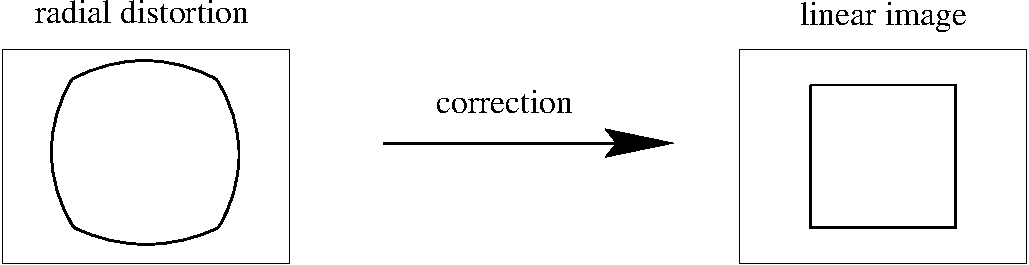
\includegraphics[width=\textwidth]{distortion_1}
    					\caption{Example of radial distortion of a square being corrected \protect\cite{book:multiViewGeo} {\label{fig:distortion}}}
    				\end{center}
				\end{figure}				
				It is caused by the fact that different areas of a lens have slightly different focal lengths \cite[p. 42]{book:modern}.
				There is a lot of information available on how distortion happens so only the basics will be covered here. %, however some reading suggestions are (READING SUGGESTIONS HERE).
				The fundamental stages of processing images for use in computer vision are based on geometry.
				To reliably calculate depth in a scene, the system needs to know the intrinsic %and extrinsic 
				parameters of a camera.
				Essentially, the system wants to know if what the camera is producing is a true representation of the scene it is recording.
				Much like when you make a visit to see an optician. 
				The optician will carry out a process to try and discover if what you see is a distortion of reality.
				The parameters will allow the system to take the images and pre process them (undistort) so that it can be confident they are true.
				This is done by producing both a camera geometry and a lens distortion model through a process of calibration.  
				The two models will now be discussed in a little more depth.				
				%more depth here
				\subsection{Camera Model}
				Most of the information available on camera models are focused around a pinhole camera.
				The following description and figures of this model is taken from \citeasnoun[p. 371-373]{definition:cv}, If more depth is needed I advise you read the cited material.
				The pinhole camera model is the most basic type of camera, that still holds the fundamental mathematics on how most modern digital cameras work today.
				\begin{figure}[!ht]
				\begin{center}
					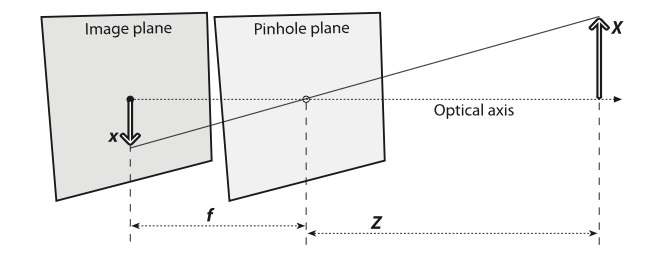
\includegraphics[width=\textwidth]{pinhole}
					\caption{Pinhole camera model as shown in \protect\citeasnoun[p. 372]{definition:cv} {\label{fig:pinhole}}}
				\end{center}
				\end{figure}
				In a pinhole camera (See Figure \ref{fig:pinhole}) light reflected from the scene/object travels through a pinhole that is made in the pinhole plane.
				This light then gets projected onto the image plane.
				The size of this projected image is proportional to the focal length $f$.
				Where $Z$ is the distance from the pinhole plane to the object, $X$ is the length of the object and $x$ is the objects image on the image plane.
				Therefore we can work out the size of the object using the equation $-x=f\dfrac{X}{Z}$.
				For mathematical simplification \citeasnoun{definition:cv} states that the negative value can be ommited leaving $x=f\dfrac{X}{Z}$.
				This is done by moving the image plane in front of the pinhole plane, and then treating the pinhole as a center of projection (See Figure \ref{fig:pinhole2}).
				This results in an image that is the correct way up. However it would be impossible to make this camera physically, it is simply to make the mathematics less complicated.
				\begin{figure}[!ht]
				\begin{center}
					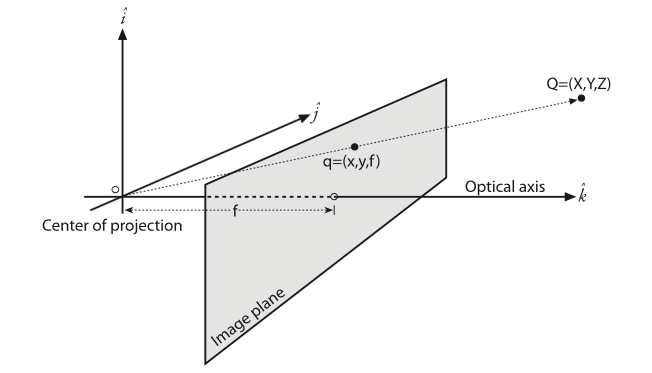
\includegraphics[width=\textwidth]{pinhole2}
					\caption{Pinhole camera model with image plane in front, as shown in \protect\citeasnoun[p. 372]{definition:cv} {\label{fig:pinhole2}}}
				\end{center}
				\end{figure}
				%THIS ASSUMES KNOWLEDGE ON HOW A CAMERA WORKS
				In the real world, the center of projection will not be precisely in the middle of the imaging sensor of a camera.
				Therefore displacement values need to be considered, $c_{x}$ and $c_{y}$.
				The resulting model allows us to pinpoint the point $Q$ (a point in real space) with coordinates $(X,Y,Z)$ as a pixel location (a point on the image) where the pixel location is $(x_{screen}, y_{screen})$.
				This results mathematical model of $x_{screen}=f_{x}\left(\dfrac{X}{Z}\right)+c_{x}$, $y_{screen}=f_{y}\left(\dfrac{Y}{Z}\right)+c_{y}$.
				Having a model like this allows us to define the parameters of the camera so that false transformations of light being collected from the physical world can be corrected.
				%MAYBE ADD SOME MORE STUFF ABOUT PIXEL MATCHING HERE
				This is important for methods of image rectification which will be discussed later.
				\subsection{Lens Distortion}
					The camera models discussed assume that cameras produce images in which the straight lines represent the same straight lines that are in the scene.
					However as discussed earlier a lens is never perfect and so many will create a visible curvature in the projections of straight lines in an image.
					Unless this distortion is taken into account, it becomes impossible to create highly accurate photorealistic reconstructions.
					A phenomenon known as radial distortion produces a visible curvature on the straight lines that appear in the image.
					This is where pixels in the image are displaced away or towards the image centre by an amount proportional to their radial distance.
					These types of distortion are known as barrel and pincushion respectively.
					The Leap Motion has a radial distortion, more specifically it is known as a fisheye.
					The fisheye is a distortion where the image that is produced provides an near 180\degree span side-to-side \cite{book:sam}.
					
				\subsection{Image Rectification}
				 TODO
				
			\section{Classification}
				\begin{quote}
					\textit{A classifier is a procedure that accepts a set of features and produces a class label for them.}
					\cite[p. 487]{book:modern}
				\end{quote}
				Classifiers are like rules, data gets passed in, in this case a feature in an image, and the rule returns a class label.
				There are three basic ingredients to the recipe of classification.
				\begin{enumerate}
					\item{Find a labelled dataset.}
					\item{Build the features from within the dataset.}
					\item{Train the classifier with the features.}
				\end{enumerate}
				The most difficult ingredient to apply is building the features.
				Some feature constructions are more suited to certain applications than others.
				It is important to extract the features that show the variation between each class, as opposed to extract the features that show the variation within a class.
				As an example, one might want to extract the features of a car and the features of a van.
				The only features that are important are the ones that differentiate between a car and a van.
				The features that differentiate between one car and another variation of a car are not important.
				On the other hand, it is clear to see there might also be a use for differentiating between two different cars in another scenario.
				Showing that extraction of these features is very much application dependant.
				
				\subsection{Extracting Image Features}
					\subsubsection{Edge Detection}
					In many cases, the first stage of image analysis is to determine where the edges are.
					Evidence suggests that edge detection is an important part of biological vision, particularly in mammals.
					In most situations a predator (or prey) can be seen to be contrasted sharply with its background.
					By noting the edges enables the animal to quickly recognise other animals near it.
					Which explains why camouflage is such a popular technique in the animal kingdom \cite{book:aiIlluminated}.
					An object is separated from its background in an image by an occluding contour.
					An occluding contour is a line where, on one side, the pixels in the image lie on the background, and on the other side, lie on the object.
					Occluding contours form the outlines of objects.
					Edges can be obtained from large image gradients.
					Such as those cause by sharp changes in brightness.
					\subsubsection{Corner Detection}
					The terms "feature", "corner" and "image point" are used interchangeably throughout literature.
					For example \citeasnoun[p. 317]{definition:cv} describes corners as
					\begin{quote}
						``\textit{the points that contain enough information to be picked out from one frame to the next.}''
					\end{quote}
					Where as, \citeasnoun[p. 179]{book:modern} describes corners as a local area where the orientation of the image gradient changes sharply; a corner in the more literal sense of the word.
					\citeasnoun{book:modern} says a corner is a more specific term of something that can be described as an image point.
					This report will continue using the term corner as \citeasnoun{definition:cv} has, so as to avoid confusion with any code references in OpenCV later on.
					
					Corners are easy to match between different images.
					This makes them extremely useful when reconstructing points in three dimensions when using multiple images.
					Such as the images produced in stereopsis.
					The idea is to extract unique points in an image that can be tracked in another image of the same object or scene.
					Imagine picking a point on a large blank wall in one image, it wont be very easy to find the exact same point in the second image.
					Instead unique points should be selected.
					Such as a tap sticking out of the wall.
					
				\section{Summary}
	%----------------------------------------- Chapter 3 -----------------------------------------%
	\chapter{Requirements Analysis}\label{chap:req}
	\section{Introduction}
	This chapter attempts to lay out a set of requirements for the framework, from the point of view of the stakeholders.
	They will set out a contract between the stakeholders and the framework developer as a means to show what the framework is going to be. It should \textbf{not} show how it will be done - that is the purpose of design \cite{book:dawson}.
	They provide goals upon which a realistic scope for the project may be set and will also be the backbone of the tests that are to be written during implementation.
	
	The elements needed to produce a good requirements analysis are as follows.
	\begin{itemize}
		\item \textbf{Stakeholder identification} is important so that the requirements are of use to who they are being developed for.
		\item \textbf{Use case analysis} identifies interactions between your system and users or other external systems. Also helpful in mapping requirements to your systems \cite{book:uml}.
		\item \textbf{Functional requirements} of a system define the system, the data and the user interface \cite{book:dawson}.
		\item \textbf{Non-functional requirements} should lay out constraints, standards, limitations, performance requirements, verification requirements and validation criteria~\cite{book:dawson}.
		\item \textbf{MoSCoW Prioritisation} will set the prioritisation for each requirement. This gives a good identification as to which ones should be developed first.
	\end{itemize}
	The next few sections will elaborate on these and show the documentation produced. 
		
		\section{Stakeholder Identification}
			This project is aimed at producing an open source framework that will suit a variety of users, with the main focus being on the \textit{application developer}, where the \textit{application developer} will use the framework to develop other applications.
			The framework being developed here will not be an application that can be used as an end user.
			It will be designed to be a simple-to-use interface that saves the \textit{application developer} a large amount of time when applying it to their own application.
			However, it is possible that other applications might need access to information that is produced by the framework, therefore another actor of \textit{user} needs to be considered.
			Through the analysis of existing libraries and solutions that work with other imaging systems, it is possible to identify what would be suitable to provide as a simpler solution for the leap motion.
			The stakeholder also plays a major role in discovering and keeping a project, within a defined scope.
			As the \textit{application developer} will be the main user of the system, they will	have most of the interactions.
			
			In summary, the stakeholders are
			\begin{description}
			\item[Application Developer] who will have the most interactions with the system.
			\item[User] who will in most cases be an external system.
			\end{description}
		
		\section{Requirements Capture}
			Due to the exploratory nature of this project, it is hard to realise what is fully required of the system at this stage.
			However, the research carried out in chapter~\ref{chap:background} can give a guide as to what might be needed.
			The requirements caught here can then be explored in the first iteration and then then expanded upon during the design stage of the next iteration.
			The problem now is to capture what requirements need to be in place to create the framework.
			In chapter~\ref{chap:background} four steps were defined to achieve successful correspondence between images.
			In summary these were:
			\begin{enumerate}
				\item Remove distortion from the images.
				\item Rectify the images.
				\item Find corresponding features in the images and produce a disparity map.
				\item Turn the disparity map into distances and produce a depth map.
			\end{enumerate}
			However, it is arguable to say that these steps are for quite a specific problem, and a framework should be more generic.
			Therefore this framework should be able to carry out all of the operations above, without any dependency on the previous step.
			The application developer should be able to carry out manipulation on the images separately from the images that are getting processed through the algorithms in OpenCV.
			This will allow for the development of an application that might show a before and after image for example, rather than only having access to an image post processing, that might have become non-understandable to a human.
			
			For classification it will be useful to be able to train the classifier.
			It will also be useful to be able to change the parameters that define the classifier.
			This data should have the ability to be reset, on a new set of data.
			
			The ability to remap the pair of two dimensional images into a three dimensional form will be used to explore classification methods.
			
		\section{Use Case Analysis}
		This section has been produced by following the methods outlined by \citeasnoun{book:uml} in ``\textit{Learning UML 2.0}''.
			\subsection{Use Case Diagram}
			
			\begin{figure}[ht]
			\begin{center}
    				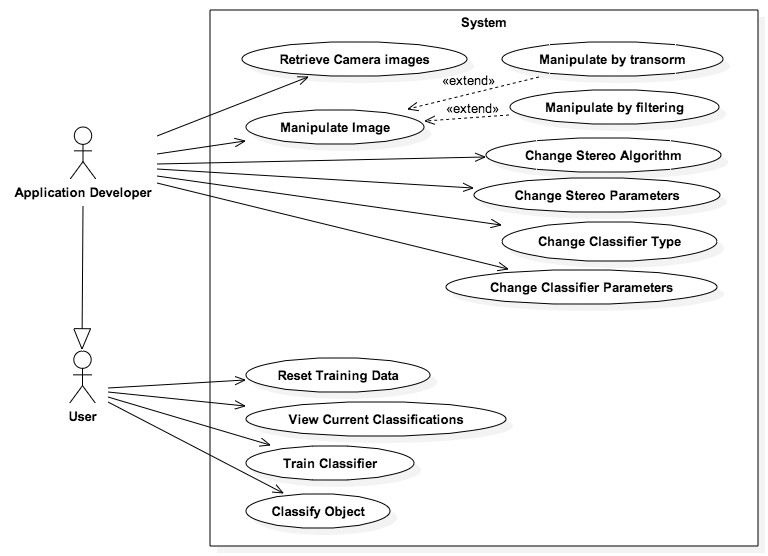
\includegraphics[width=\textwidth]{use_case_2}
    			\caption{UML use case diagram \protect {\label{fig:use_case_1}}}
    			\end{center}
			\end{figure}	
			A use case diagram is used to capture pieces of functionality that a system will provide to the stakeholder and other users.
			Figure~\ref{fig:use_case_1} is an example of a UML use case diagram.
			The stick figures represent actors on the system, the ovals represent use cases and the box enclosing the use cases show the overall system. 
			The actors are acting upon the system through the means of a use case.
			Each connecting line shows the use case upon which the actor should be able to interact.
			In the case of a line between use cases that shows the ``\textit{extend}'' relationship, it shows that the use case might want to completely reuse the connected use cases behaviour.
			However in \textit{UML 2.0} this reuse is optional and dependent on a runtime or system implementation decision.
			Remember at this stage we should not be stating \textbf{how} it should be implemented.
			\subsection{Use Case Description}
			Table~\ref{tab:use_retrieve_camera_images} is one example of a use case description.
			A use case description provides the reader a little more insight into what actions are going to be performed.
			This is not always immediately clear from the higher level use case diagrams.
			Each use case that has been defined so far, has a corresponding use case description.
			These can be found in appendix~\ref{app:use_case_descriptions}.
			\begin{table}[h]
\begin{tabular}{|p{1.5in}|p{3.4in}|}
\hline
\varusecase         & \texttt{RetrieveCameraImages}                                                                                                        \\ \hline
\vardescription     & The application developer must have access to raw camera images to use with other elements of the library. It will also allow for the images to be displayed. \\ \hline
\varactor           & Application developer \\ \hline
\varentry           & The library and the system it is being used on, must have the relevant dependencies loaded and the leap motion controller connected. \\ \hline
\varflow            & \begin{enumerate}
                        \item Application developer requests an image
                        \item Library checks leap motion is ready
                        \item Library retrieves image from \texttt{LeapSDK}
                        \item Library converts image to usable format
                        \item Library returns image
                      \end{enumerate} \\ \hline
\varaltflow         & If leap motion controller is not ready , library throws \texttt{leapNotFound} exception. \\ \hline
\varexit            & Application developer receives valid image. \\ \hline
\end{tabular}
\caption{Documented \texttt{RetrieveCameraImages} use case \protect {\label{tab:use_retrieve_camera_images}}}
\end{table}
		\clearpage
		\section{Functional Requirements}
			
			As this is a framework, user interface requirements do not need to be considered.
			\begin{description}
				\item[Automatic camera configuration.] The framework should abstract the leap motion configuration away from the application developer and should not require any explicit calibration.
				\item[Default configuration.] The framework should have a default configuration for training and classifying three dimensional shapes.
			\end{description}
				
			
		\section{Non-Functional Requirements}
			\begin{description}
				\item[Speed.] The framework needs to be able to process images and return a useful classification output in near real-time. 
				A minimum of 15 frames per second should be the target.
				\item[Accuracy.] The framework should have equal to or greater than 90\% accuracy in its classification ability.
				\item[Multi-platform.] The framework should be usable on all of the platforms that the leap motion is currently supported on.
				\item[Java standards] The framework should conform to Java standards and have a well documented interface.
				A Javadoc should be produced.
				\item[Semantics.] The framework should not stray too far from terminologies and semantics used within existing computer vision libraries, unless it is essential. Ensuring users with prior experience of computer vision can use it with ease.
				\item[Extensibility.] As the project will be made open source, the framework needs to be designed with extensibility in mind.
			\end{description}
			
		\section{MoSCoW Prioritisation}
			MoSCoW is a recognised method for prioritising requirements by their importance. \citeasnoun{book:moscow} defines the categories in order of highest to lowest importance as
			\begin{description}
				\item[Must have. ] All features categorised in this group must me implemented for the system to work.
				\item[Should have. ] Features categorised in this group are of high importance but are not essential to the system working.
				\item[Could have. ] These features will enhance the system by giving it greater functionality, but they do not have to be delivered as a priority.
				\item[Want to have. ] These features only apply to a small group of users and have limited business value.
			\end{description}
			The terminology here has a business system feel.
			Where the term \textit{business value} is used above, in terms of this project it will just mean a limited value to the libraries end result.
			Table~\ref{tab:moscow_table} shows the user stories with their recognised priority.
			% Please add the following required packages to your document preamble:
% \usepackage{multirow}
\begin{table}[h]
\centering
\begin{tabular}{|l|c|c|c|c|}
\hline
\multicolumn{1}{|c|}{\multirow{2}{*}{Task}} & \multicolumn{4}{c|}{MoSCoW Prioritisation} \\ \cline{2-5} 
\multicolumn{1}{|c|}{}                      & Must     & Should     & Could    & Wont    \\ \hline
Retrieve camera images                      & x        &            &          &         \\ \cline{1-1}
Manipulate image                            & x        &            &          &         \\ \cline{1-1}
Manipulate by transform                     &          & x          &          &         \\ \cline{1-1}
Manipulate by filtering                     &          & x          &          &         \\ \cline{1-1}
Reset training data                         &          & x          &          &         \\ \cline{1-1}
View classification                         &          & x          &          &         \\ \cline{1-1}
Classify new object                         &          &            & x        &         \\ \cline{1-1}
Classify image                              &          &            & x        &         \\ \hline
\end{tabular}
\caption{MoSCoW task prioritisation\protect {\label{tab:moscow_table}}}
\end{table}


			\clearpage
			The prioritisations have been worked out so that the fundamental elements of the framework will get created first.
			Although the end product should be able to classify images, there is not yet a guarantee that it is possible to do so.
			All of the previous requirements have to be implemented before any type of classification can be considered.
		\section{Summary}
			The initial requirements for the system have now been identified.
			Now this is completed an initial design can be created.
			This design will be shown in prototype 1 of chapter~\ref{chap:des&imp}.
			Chapter~\ref{chap:des&imp} will make use of these requirements.
			It will aim to build upon them and turn them into a working system.
    		
	
	%----------------------------------------- Chapter -----------------------------------------%
	\chapter{Design, Implementation and Testing}\label{chap:des&imp}
	\section{Introduction}
	This chapter covers the implementation stage of the project.
	In chaper \ref{chap:introduction} the methodology of how this was going to be done was outlined.
	The implementation has been planned in three iterations.
	Where the first iteration is a throwaway prototype and the further two iterations will follow the evolutionary prototype method.
	Each iteration will be further broken down into work items.
	The work items are loosely based on the initial requirements defined in chapter \ref{chap:req}.
	These might changed slightly based on the evaluation carried out in each iteration.
	\clearpage
	\section{System Architecture}
	\begin{figure}[ht]
			\begin{center}
    			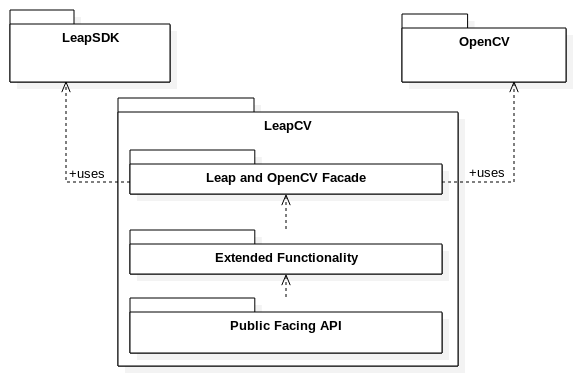
\includegraphics[width=\textwidth]{system_architecture_2}
    			\caption{High level system architecture \protect {\label{fig:system_arch_1}}}
    		\end{center}
			\end{figure}	
			
			Figure~\ref{fig:system_arch_1} outlines the intended architecture of the framework.
			\begin{description}
			\item[Leap and OpenCV Facade] This will bring the two libraries, being OpenCV and the LeapSDK, together.
			This is where most of the utility style functionality will sit.
			\item[Extended Functionality] This is where the functionality of each library will be put to use.
			Higher level functionality such as classification and object detection will sit here.
			\item[Public Facing API] The framework will provide a public facing API that will ensure that the library is simple to use.
			All of the complex functionality will be occurring in the private packages.
			\end{description}
			\clearpage
	\section{Pre-Requisites for Implementation}
		Before any implementation can take place the environment needs to be set up.
		The Java 1.8 SDK should be installed on the platform that is being developed on, ensuring that it is a version with JavaFX support.
		IntelliJ IDEA should be installed on the platform that is being developed on.
		JUnit comes as a standard package with IntelliJ IDEA.
		
		The latest version of OpenCV should be downloaded from the website\footnote{\url{http://www.opencv.org}}.
		Instructions for installation are also available there.
		It is important to ensure that OpenCV has been compiled with the Java bindings so the instructions have to be followed carefully.
		Once installed the library should be imported to the project. %METHOD HERE 
		Once imported, to ensure the native libraries get loaded when the project gets built it is important to include the line in listing \ref{lst:code_1}.
		
		\lstinputlisting[caption=Loading the OpenCV Library into the Project, label=lst:code_1]{main.java}		
		The LeapSDK is available from the leap motion website\footnote{\url{http://developer.leapmotion.com}}.
		The methods for importing the LeapSDK into the project are also found here.
	\section{Iterations}
		The next few sections will talk in depth about the key work items that were completed to produce the prototype in each iteration.
		Below is a description of what will be found in each section.
		\begin{description}
		\item[Design] will show the design that has been used in the implementation and highlight any key changes through discussion.
		\item[Implementation] will be split into stages to highlight the thought process that went into developing the library.
		\item[Test] will describe the unit tests and any key results that might have an effect on further decisions to be made.
		The tests will be split into:
			\begin{itemize}
				\item \textbf{Performance tests} These will be used to test some of the non-functional requirements such as the frame rate. 
				It must be noted that these tests are specification dependant and will therefore vary machine to machine.
				These tests will only be run on the basic specification MacBook Pro 13inch Version 8,1.
				An example of a performance test written in JUnit can be seen as a listing in appendix~\ref{lst:code_8}.
				\item \textbf{Unit tests} These will be used to test the program throughout development, any unit tests carried over into another iteration will also act as a form of regression test, though regression testing wont be explicitly carried out due to time constraints.
				\item \textbf{Acceptance tests} These are previously defined tests, based on the use case analysis.
				They will provide a measure as to how far the solution has gone to solving the initial problem.
			\end{itemize}
		\item[Evaluation] will review how that iteration went and what work needs to be completed or changes made before moving into the next one. It will be broken down into ``what went well'', ``what went badly'' and ``lessons learned''.
		\end{description}
	\section{Prototype 1}\label{sec:p1}
		\subsection{Design}
		The first implementation will be based on the requirements that were discovered in chapter~\ref{chap:req}.
		This iteration is a throwaway prototype, with the idea of exploring the functionality of the libraries, so as to elicit more requirements.
		These will be discussed in the evaluation section later in prototype~\ref{sec:p1}.
		The knowledge gained through this prototype will then be applied to the first of the evolutionary prototypes, prototype~\ref{sec:p2}.
		\subsection{Implementation}
		\subsubsection{Stage 1 - Retrieve Images From the leap motion}
		The first stage involves gaining an understanding of what type of images can be received from the leap motion.
		The type \code{Image} in package \code{com.leapmotion.leap} has some useful publicly visible methods at its disposal.
		\code{Image.data()} returns a \code{byte[]} where each individual \code{byte} is a pixel in the image.
		Each \code{byte} holds an \code{8-bit} intensity value for the pixel, in integer form this is between 0(black) and 255(white).
		The \code{byte[]} is of length \code{Image.width() * Image.height()}.
		
		The example in listing~\ref{lst:code_2} shows how the \code{Image} is converted into a \code{BufferedImage}.
		Now that this is understood the first image can be retrieved from the leap motion.
		A \code{Controller} must be initialised, from this we can retrieve a \code{Frame}.
		The \code{Frame} contains an \code{ImageList} which contains an \code{Image} for both the left and the right camera.
		To ensure the images can be retrieved from the camera the \code{PolicyFlag.POLICY\_IMAGES} must be set on the \code{Controller} object.
		
		Listing~\ref{lst:code_3} is a simplified version of writing the images to two files.
		It makes use of the converter defined in listing~\ref{lst:code_2}.
		An example of one of these images is shown in figure~(INSERT FIGURE HERE). %FIGURE HERE
		%\clearpage
		\lstinputlisting[caption=Convert an \code{Image} into a \code{BufferedImage}, label=lst:code_2]{toBufferedImage.java}	
		\lstinputlisting[caption=Write \code{ImageList} to a \code{File}, label=lst:code_3]{imageWrite.java}	
		\subsubsection{Stage 2 - Distortion Removal}
		Now that the \code{Images} can be successfully taken from the leap motion, the distortion must be removed.
		The LeapSDK provides the \code{Image.warp()} method for this, however the documentation states that it is not suitable for processing full images.
		They suggest that using a shader program with OpenGL is faster.
		As this would allow the process to run on a GPU.
		However at this stage it is more interesting (and valuable to proving the hypothesis) to see whether a disparity map can be produced using OpenCV.
		Therefore, for now, the slow method will suffice.
		The listing as appendix~\ref{lst:code_4} shows the method by which this was done.
		This method then results in an image as shown in figure~(INSERT FIGURE HERE).
		Unfortunately it seems that during the process of distortion removal, some of the resolution of the \code{Image} has been lost.
		We can see this from the black pixels that are left around the outside of the \code{BufferedImage} that has been given here.
		
		\subsubsection{Stage 3 - Further Removal of Distortion with OpenCV}
		OpenCV provides functionality to resize and crop images.
		Therefore here we shall explore the further removal of distortion using OpenCV.
		In OpenCV, the type \code{Mat} in package \code{org.opencv.core} is described as ``The Basic Image Container'' in the documentation\footnote{\url{http://docs.opencv.org}}.
		The \code{Mat} is a matrix, with the same width and height of the image.
		Each location in the index holds an intensity value for the pixel.
		Fortunately, as previously seen, the LeapSDK provides a \code{byte[]} of pixel values.
		The images are also grey scale, meaning that they are single channel.
		Therefore there is less complexity in the storage of the image in a \code{Mat} due to there being only a single integer between the values 0 and 255 representing a pixel in a grey scale image.
		In comparison, a colour image has three (sometimes four if including alpha) channels of colour at any pixel location.
		These channels being red, green and blue (RGB).
		Each one with a value between 0 and 255.
		It is actually fortunate that the images are already grey scale, as it seems that algorithms used in feature detection, favour the use of grey scale images.
		Listing~\ref{lst:code_5} shows the method used to convert the \code{Image} into a \code{Mat}.
		\lstinputlisting[caption=Convert \code{Image} type to \code{Mat} type, label=lst:code_5]{convertToMat.java}
		Now that the image is in a \code{Mat} format it can be resized.
		This is done using the \code{resize()} method provided by the class \code{Imgproc} in the package \code{org.opencv.imgproc}.
		\code{Imgproc} is the class that handles the majority of the image processing functionality within OpenCV.
		The crop is performed by passing a region of interest to the method \code{submat()} provided by the \code{Mat} to be cropped, then storing the returned value in a new \code{Mat}.
		The region of interest is a \code{Rect} object which is a rectangle that consists of a width, a height and a pair of coordinates, at which the top left of the rectangle should begin.
		This is quite a generic process to carry out on images and can be viewed in appendix~(INSERT APPENDIX HERE).
		The end result is an image that looks like that in figure~(INSERT FIGURE HERE).
		
		\subsubsection{Stage 4 - Stereo Correspondence}
		OpenCV provides stereo correspondence functionality in the \code{org.opencv.calib3d} and the \code{org.opencv.contrib} packages.
		Namely \code{StereoBM}, \code{StereoSGBM} and \code{StereoVar}.
		The first two are variations of the stereo block matching method(TODO) and the later is the stereo variation method.
		\code{StereoSGBM} seems to be generally accepted as better than \code{StereoBM} in most scenarios, therefore \code{StereoBM} will not be attempted here.
		(INSERT CODE AND DESCRIPTIONS ON STEREO)
		
		\subsubsection{Stage 5 - Parameter Tweaking}
		Through the exploration of the algorithms in stage 4, it became clear that it was quite difficult to know what parameters to set to get a good disparity map from the image.
		Therefore as part of the prototyping methodology, a test bench graphical user interface (GUI) application will be made in JavaFX.
		The GUI will not only be able to allow for parameter changing at run-time.
		It will also give a good idea as to the performance that can be achieved with each of the stereo matching algorithms.
		JavaFX is a GUI framework for Java.
		It is shipped with Java 1.8 SDK and has been developed to take the place of the Java Swing framework.
		For speed of development, SceneBuilder will be used.
		SceneBuilder is a tool that allows for rapid development of GUIs.
		It allows for the drag and drop of GUI elements such as sliders onto the page and generates the underlying code.
		An example of the GUI that was quickly put together is in figure~(INSERT FIGURE HERE).
		The sliders visible are used to quickly change the stereo parameters.
		To allow for the processing to get done in real time, it was decided to make use of the \code{Listener} class within the LeapSDK.
		Then implementing an \code{ObservableValue} which is included in the JavaFX framework.
		The \code{ObservableValue} follows the observer design pattern.
		Allowing the \code{Listener} to notify the main GUI thread when there is some new data for it to display.
		The reason for doing this was so the \code{Listener} could be run on a separate thread to the JavaFX GUI.
		It is also important to allow the GUI thread to handle when to instantiate the \code{Listener}.
		Using the \code{Platform.runLater()} method.
		The \code{Listener} seems to lock the GUI thread if it is not done this way.
		This is possibly due to the fact that by default the leap motion returns images at a very high frame rate.
		This resulted in finding good parameters for the correspondence algorithms.
		\subsection{Test}
		As this prototype is intended to be thrown away, it must be noted that the testing of this prototype was not intended.
		\code{StereoVar} gave the best resulting disparity map, however, it took a lot longer to process.
		\code{StereoSGBM} gave the worst resulting disparity map but the processing time was a lot faster.
		However it needs to be considered that the slow method of distortion removal was implemented here.
		\subsection{Evaluation}
		\subsubsection{What went well?}
		The first prototype allowed for a good exploration of the OpenCV library.
		A vast amount of knowledge was gained as to how the library works.
		This will be useful in the next iteration.
		\subsubsection{What did not go so well?}
		Using the \code{Listener} seemed to make the code a lot more complex to work with.
		It seems more suited to applications that are heavily making use of the LeapSDK with its tracking functionality alone.
		In this case it is believed it would be better to access the images, by explicitly requesting them from the leap motion.
		This will make it a lot simpler for development as each image needs to be processed individually.
		The \code{Listener} is intended for use when the camera is working at it highest frame rate.
		However through the frame rate results we have here, we can see that it will never be working at full capacity with the methods intended to be used.
		%After completion, there are a few requirements changes that will be considered.
		\subsubsection{Lessons learned?}
			In stage 2 of this iteration, it was suggested that the slow method was going to be used for distortion removal, as speed was not important at this stage.
			Going into the next iteration, an attempt should be made at optimising the process.
			This is due to the fact using the slow method did indeed have a large hit on the frame rate.
	\section{Prototype 2}\label{sec:p2}
		\subsection{Design}
		\subsubsection{Class Diagram}
		The class diagram shown in figure~\ref{fig:class_diagram_it_2} is a basic model of the system that is going to be built upon.
		\begin{figure}[ht]
		\begin{center}
    			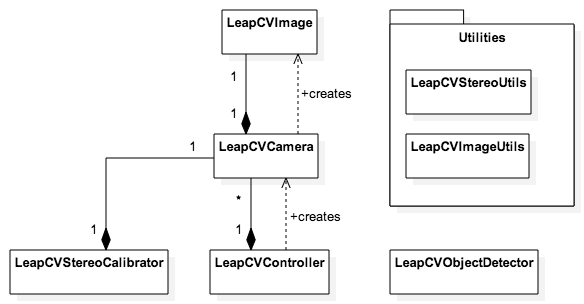
\includegraphics[width=\textwidth]{class_diagram_it_2}
    			\caption{Class Diagram for Prototype 2 \protect {\label{fig:class_diagram_it_2}}}
    		\end{center}
		\end{figure}			
		Each class was identified using the CRC process. (CITE)
		CRC stands for Classes Responsibilities and Collaborations.
		The cards contain three sections of information about a single class.
		These are:
		\begin{itemize}
			\item \textbf{Class:} The name of the class.
			\item \textbf{Responsibilities:} The information the class owns and the functionality it performs.
			\item \textbf{Collaborations:} The classes that this class also interacts with.
		\end{itemize}
		\input{crc_LeapCVController}
		The CRC for each class can be found in appendix~\ref{app:crc_diagrams}.
		The \code{Utilities} package will be where most of the extended functionality will sit.
		\subsubsection{Requirements Changes}
			Now that much more knowledge has been gained surrounding the OpenCV library, it has been decided a few changes will be made to the requirements of the framework.
			To simplify the use of the framework, and keep the project within scope, it has been decided that the image manipulation functionality will be handled by the framework.
			Meaning that the application developer can request either, the original image, or the undistorted image that the framework has defined.
			This will avoid complications in having to handle differently sized images.
			It will also keep the framework within a certain performance boundary.
			Block matching algorithms work faster on lower resolution images; if an application developer resized an image to become larger than it was originally, then requested a disparity map, the framework performance will decrease.
			The new use case diagram reflecting these changes can be seen in figure~\ref{fig:use_case_2}.
			
			\begin{figure}[ht]
			\begin{center}
    				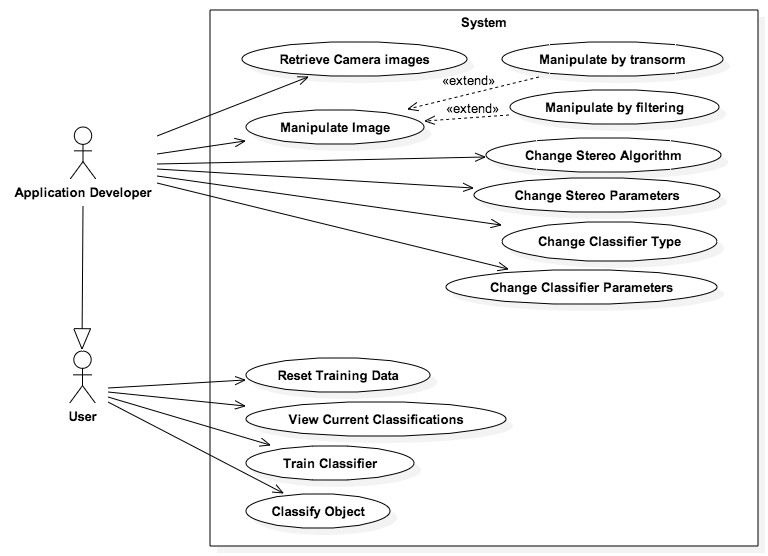
\includegraphics[width=\textwidth]{use_case_2}
    			\caption{New UML use case diagram \protect {\label{fig:use_case_2}}}
    			\end{center}
			\end{figure}	
		\subsection{Implementation}
		\subsubsection{Stage 1 - The Basis of the Framework}
			As the framework is designed to be extended upon by other application developers, it is useful to think about the way in which it will be deployed.
			The framework should be IDE independent.
			The application developers using it should be able to easily import the framework into their own project.
			All they will need is the source code being developed here, and the OpenCV and LeapSDK dependencies to be satisfied.
			To do this a Git repository will be made that holds the source for the framework.
			The Git repository will have nothing but Java related files.
			None of the files should be related to any individual IDE.
			%The documentation below will then describe how the project can be imported.
		\subsubsection{Stage 2 - Refactoring Based on New Design}
			Now that the design has been created, it will be useful to create the templates for each class.
			Also sometimes known as the skeleton classes.
			It is also the case that some of the functionality from prototype 1 can be transferred into the new utilities classes.
			Primarily the segments of code that were used to manipulate and convert the images.
			This functionality will be heavily tested within this iteration, providing a reliable foundation on which to build the rest of the system.
			
		\subsubsection{Stage 3 - Distortion Removal Optimisation}
			As highlighted at the end of the previous iteration, it was suggested that during this iteration the distortion removal process should be optimised.
			The method that is currently used, calls the \code{warp()} method from the LeapSDK \code{Image} class.
			This method is, through self admittance by leap motion, a non optimised way to remove image distortion.
			They suggest that only a few image pixels should be used.
			However, in this scenario it is required that the entire picture gets used, so that it can be further processed in OpenCV.
			The \code{Image} class also has \code{distortion()} method.
			This method contains the calibration map for the leap motion.
			It was suggested by \citeasnoun{blog:leap} that these values can be used with the \code{remap()} function in OpenCV.
			\citeasnoun{blog:leap} does state that there is no guarantee that this method is correct.
			With this method, the distortion map is loaded at the initialisation of the leap motion.
			This data is set in the factory, or when the leap motion is explicitly calibrated within its separate settings application.
			Unless the leap motion is going through the calibration process, this distortion map does not change.
			Once the distortion map is loaded at initialisation, it can be passed with a \code{Mat}, to the \code{remap()} method.
			The code provided by \citeasnoun{blog:leap} is written in the Python programming language, so analysis is required to port it over to Java.
			The method provided by OpenCV is highly optimised with the library, and the processing time has been noticeably decreased.
			Listing~\ref{lst:code_5} shows the method by which the distortion \code{Mat} has been initialised.
			The values that get returned are placed into the \code{LeapCVCamera} class.
			This method is quite similar to the code in listing~\ref{lst:code_4}.
			It still uses the \code{warp()} method however this slow method is only used once throughout the run time of the using the LeapCV framework.
			Rather than every time a frame is loaded as in iteration 1.
			\lstinputlisting[caption=Initialisation of Distortion Data, label=lst:code_5]{initialiseDistortionMats.java}
		\subsection{Test}
			\subsubsection{Performance Tests}
			\begin{table}[h]
\centering
\begin{tabular}{|l|l|l|l|}
\hline
\textbf{Test} & \textbf{Minimum Value} & \textbf{Actual Value} & \textbf{Pass}
\\ \hline
getImage                  & 15 FPS                 & 1112 FPS            & Yes           \\ \hline
getImageUndistorted       & 15 FPS                 & 144 FPS             & Yes           \\ \hline
getDisparityStereoVar     & 15 FPS                 & 11 FPS              & No            \\ \hline
getDisparityStereoBM      & 15 FPS                 & 87 FPS              & Yes           \\ \hline
getDisparityStereoSGBM    & 15 FPS                 & 42 FPS              & Yes           \\ \hline
getPointCloud             & 15 FPS                 & 11 FPS              & No            \\ \hline
\end{tabular}
\caption{Results of First Frame Rate Performance Test (FPS = Frames Per Second)\protect {\label{tab:performance_1}}}
\end{table}

\textbf{\textit{Notes on table \ref{tab:performance_1}:}}
\begin{description}
	\item[getImage] The value in a single test varied between 800 - 1500 FPS.
	Over 20 tests it averaged out.
	\item[getDisparityStereoVar] This was below the minimum required value, however it produces the best disparity map.
	This test can be passed, but not without sacrificing disparity map quality.
	\item[getDisparityStereoSGBM] It was noted that after 10 consecutive runs of this process, the frame rate dropped dramatically.
	It was discovered this was due to a memory leak.
	Each time the method \code{getDisparityStereoSGBM()} gets called, a new StereoSGBM object is instantiated within the method scope. From the frame rate measurement we can assume that this happens 42 times per second and is therefore processor intensive. This was not leaving enough time or resource for the Java garbage collector to free the used memory. Although the test has not failed, this needs to be optimised as it causes the machine to become unresponsive.
	\item[getPointCloud] This uses the StereoVar method with the default parameters and thus is bottlenecked by StereoVar.
	This test can be passed, but not without sacrificing the point cloud quality.
	
\end{description}
			
			\subsubsection{Unit Tests}
			\subsubsection{Acceptance Tests}
			\begin{table}[h]
\centering
\begin{tabular}{|l|l|l|}
\hline
\textbf{Test Reference} & \textbf{Pass} & \textbf{Notes} \\ \hline
1              & Yes              &                \\ \hline
2              & Yes              &                \\ \hline
3              & Yes              &                \\ \hline
4              & Yes              &                \\ \hline
5              & No              & Not yet implemented               \\ \hline
6              & No              & Not yet implemented               \\ \hline
7              & No              & Not yet implemented               \\ \hline
8              & No              & Not yet implemented               \\ \hline
9              & No              & Not yet implemented               \\ \hline
10             & No              & Not yet implemented               \\ \hline
\end{tabular}
\caption{Acceptance Test Template \protect {\label{tab:acc_test_1}}}
\end{table}
		\subsection{Evaluation}
			\subsubsection{What went well?}
			The optimisation of distortion removal was successful.
			Refactoring made the framework a lot easier to use and develop.
			Creating a Git repository was easily done and will allow for a simple release of the open source framework.
			\subsubsection{What did not go so well?}
			\subsubsection{Lessons learned?}
	\section{Prototype 3}\label{sec:p3}
		\subsection{Design}
			\subsubsection{Class Diagram}
			\begin{figure}[ht]
		\begin{center}
    			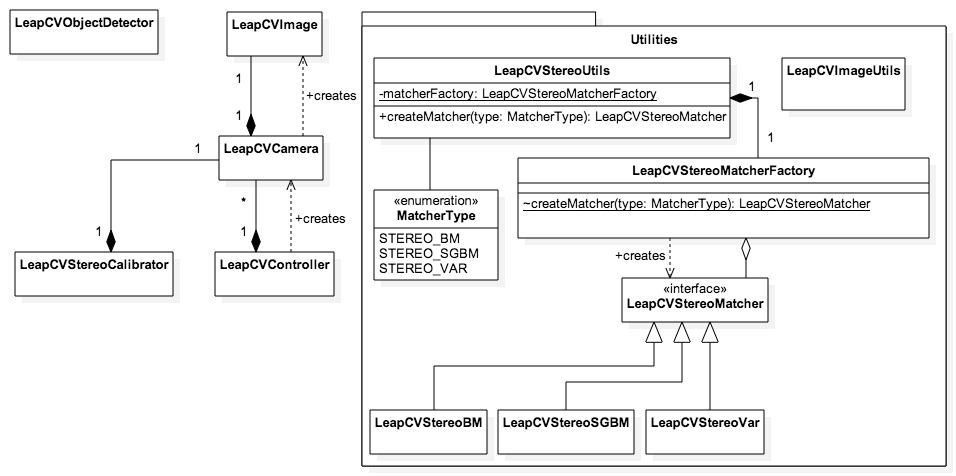
\includegraphics[width=\textwidth]{class_diagram_it_3}
    			\caption{Class Diagram for Prototype 3 \protect {\label{fig:class_diagram_it_3}}}
    		\end{center}
		\end{figure}			
			\subsubsection{Requirements Changes}
		\subsection{Implementation}
		\subsubsection{Stage 1 - Obtaining the Q Matrix}
			OpenCV requires the camera's intrinsic parameters to be known so that images can have the distortion removed, and be rectified, in a stereo set up.
			By carrying out the calibration, it gives what in OpenCV is known as the \code{Q} matrix.
			This is a 3x3 \code{Mat} that contains the distortion coefficients for the camera.
			In iteration 1 it was discovered that the images could have the distortion removed by using the distortion values that were provided by the LeapSDK.
			However the distortion coefficients are not given.
			This was not realised until this iteration.
			An attempt was made to extract the distortion coefficients from the camera by doing stereo calibration.
			However it was an unsuccessful attempt.
			The code for this attempts can be found in appendix~(INSERT APPENDIX HERE).
			Another thought is that the distortion coefficients can be calculated from the already obtained distortion map.
			A method was outlined on the internet that might prove useful by \citeasnoun{url:distortion}.
			It gives a mathematical example of how to recover the distortion coefficients from a pre calculated distortion map.
			This method is quite advanced and it will not be feasible to complete in the time-scale of this project.
			\citeasnoun{blog:leap} does provide some values obtained from calibration of the leap motion.
			However these values will vary slightly from camera to camera due to manufacturing precision as mentioned in chapter~\ref{chap:background}.
			It is therefore unlikely that the values will be exact for the leap motion in use here.
			Although for speed of development these values will be used as the \code{Q} matrix for this project.
			In hope that it will provide some form of output in the next stage.
		\subsubsection{Stage 2 - Three Dimensional Reprojection}
			The process of three dimensional reprojection is to achieve a model of the real world scene that the images represent. 
			With true distance values that are identical to the real world.
			This includes depth measurement.
			To do this with OpenCV the \code{Q} matrix is needed as described in stage 1.
			The \code{Q} matrix is made of values that allow the values in the disparity map, generated in the previous two prototypes, to be turned into true depth values.
			The result is known as a point cloud.
			The method used to generate the point cloud can be seen in listing~\ref{lst:code_6}
			\lstinputlisting[caption=Generate a Point Cloud from the Disparity Map, label=lst:code_6]{getPointCloud.java}	
			It was found that the point clouds varied greatly in quality based on the algorithm that was used to generate the disparity map.
			There was no way to test this here other than to visually inspect the output point clouds.
			The point clouds were written to file using the method in listing~(LISTING HERE).
			They were then opened in a tool called ccViewer\footnote{\url{http://www.danielgm.net/cc/}}.
			This tool allows for the visualisation of point clouds.
			An example of a point cloud using the \code{StereoSGBM} method can be seen in figure~(INSERT FIGURE HERE).
			And example of a point cloud using the \code{StereoVar} method can be seen in figure~(INSERT FIGURE HERE).
			The images show that the \code{StereoVar} Method gives a much clearer point cloud.
			However when looked at multiple angles It shows that some of the depths are non realistic.
			This might be due to the \code{Q} matrix mentioned earlier, not being the exact one for the leap motion used in this project.
			As time is running low and it is difficult to achieve a good point cloud without a good calibration method, a different approach will be made for object recognition.
			Instead of making use of the disparity map functionality, an attempt will be made using methods of feature recognition for classification.
		\subsubsection{Stage 3 - Feature Matching}
			OpenCV provides numerous classes within the \code{org.opencv.features2d} and \code{org.opencv.calib3d} packages, that are used to match features within images.
			The three important classes here are \code{DescriptorExtractor}, \code{DescriptorMatcher} and the \code{FeatureDetector}.
			Each of these classes follow the factory pattern.
			Using the \code{create()} method on each class, one is able to request an object specific to the type of algorithm that will be used to detect, extract and match the features within the images.
			An example of creating a SIFT feature extractor with a FLANN matcher can be seen in listing~\ref{lst:code_7}.
			\lstinputlisting[caption=Creating Detector\, Extractor and Matcher from Factories, label=lst:code_7]{constructorLeapCVObjectDetector.java}
			This constructor makes it easy to swap the algorithms used to find the optimal one for object detection with the leap motion.
			All that needs to be changed is the flag that is passed into the \code{create()} method.
			Each algorithm type gave very different results.
			It will not be clear which one is the best type until a classifier has been implemented.
			An example of the output produced by the method in listing~\ref{lst:code_7} can be seen in figure~(INSERT FIGURE HERE).
		\subsection{Test}
			\subsubsection{Performance Tests}
			\subsubsection{Unit Tests}
			\subsubsection{Acceptance Tests}
			\begin{table}[h]
\centering
\begin{tabular}{|l|l|l|}
\hline
\textbf{Test Reference} & \textbf{Pass} & \textbf{Notes} \\ \hline
1              & Yes              &                \\ \hline
2              & Yes              &                \\ \hline
3              & Yes              &                \\ \hline
4              & Yes              &                \\ \hline
5              & No              & Not yet implemented               \\ \hline
6              & No              & Not yet implemented               \\ \hline
7              & No              & Not yet implemented               \\ \hline
8              & No              & Not yet implemented               \\ \hline
9              & No              & Not yet implemented               \\ \hline
10             & No              & Not yet implemented               \\ \hline
\end{tabular}
\caption{Acceptance Test Template \protect {\label{tab:acc_test_1}}}
\end{table}
		\subsection{Evaluation}
			\subsubsection{What went well?}
			Managed to create a point cloud, building upon successful functionality created in prototype 2.
			Managed to get features matched between images.
			\subsubsection{What did not go so well?}
			The point cloud was not of high enough quality for classifying; it was noisy and unclear.
			Time was lost looking up other options of object detection.
			\subsubsection{Lessons learned?}
	\section{Summary}
	This chapter has logged the development process of the project.
	
	It has discussed the difficulties that were faced throughout the process and highlighted the problems that were particularly interesting to overcome.
	It shows how the design has evolved over each iteration through an evaluation of the requirements.
	Moving into chapter~\ref{chap:eval}, the project as a whole will be evaluated.
	Looking at how far the project has gone in solving the original problem.

	%----------------------------------------- Chapter -----------------------------------------%
	
	\chapter{Evaluation}\label{chap:eval}
	\section{Introduction}
	In this chapter the aim is to evaluate the work that has been done toward this project.
	It will highlight which areas of work might have benefited from being done differently.
	It will also discuss how far the implementation has gone to fulfilling the original requirements.
	
	(COPY AIM AND OBJECTIVES HERE)
	
	\section{Summary}
	%----------------------------------------- Chapter -----------------------------------------%
	
	\chapter{Conclusion}\label{chap:concl}
	\section{Introduction}
	\section{Summary}
	\clearpage
	\addcontentsline{toc}{chapter}{Bibliography}
	\bibliographystyle{dcu}
	\bibliography{bibfile}
	\begin{appendices}
	\chapter{Use case descriptions} \label{app:use_case_descriptions}
			\begin{table}[h]
\begin{tabular}{|p{1.5in}|p{3.4in}|}
\hline
\varusecase         & \texttt{ManipulateByTransform} \\ \hline
\vardescription     & The application developer should be able to manipulate the image by transformation. (Such as resize or warp). For use if overriding calibration methods. \\ \hline
\varactor           & Application developer \\ \hline
\varentry           & The image needs to be instantiated and valid for a successful transformation. \texttt{RetrieveCameraImages} needs to have been successful. \\ \hline
\varflow            & \begin{enumerate}
                        \item Application developer requests a transformed image by transformation type.
                        \item Library checks image is valid.
                        \item Library validates transformation.
                        \item Library library transforms image.
                        \item Library returns transformed image.
                      \end{enumerate} \\ \hline
\varaltflow         & If the image or transformation is not valid a \texttt{TransformationException} should be thrown. \\ \hline
\varexit            & Application developer receives a transformed image as a new instance. \\ \hline
\end{tabular}
\caption{Documented \texttt{ManipulateByTransform} use case \protect {\label{tab:use_manipulate_by_transform}}}
\end{table}
			\begin{table}[h]
\begin{tabular}{|p{1.5in}|p{3.4in}|}
\hline
\varusecase         & \texttt{ClassifyObject} \\ \hline
\vardescription     & The user should be able to ask the framework to start classifying images it receives \\ \hline
\varactor           & User \\ \hline
\varentry           & The leap motion controller must be successfully calibrated and receiving valid images. The classifier must have been trained before detecting objects.\\ \hline
\varflow            & \begin{enumerate}
                        \item User requests classification of image.
                        \item Framework checks image is valid.
                        \item Framework runs object detection algorithm.
                        \item Framework returns classification of image.
                        
                      \end{enumerate} \\ \hline
\varaltflow         & If the image is not valid then the framework will notify the User. If no classification can be given then a pre defined value will be given to the user stating this.\\ \hline
\varexit            & User receives a classification for the object in the image \\ \hline
\end{tabular}
\caption{Documented \texttt{ClassifyObject} use case \protect {\label{tab:use_classify_object}}}
\end{table}
			\begin{table}[h]
\begin{tabular}{|p{1.5in}|p{3.4in}|}
\hline
\varusecase         & \texttt{ChangeStereoAlgorithm}                                                                                                        \\ \hline
\vardescription     & The application developer should be able to change the stereo algorithm used to generate the disparity map. \\ \hline
\varactor           & Application developer \\ \hline
\varentry           & The application developer should pass in a valid pre defined flag to a constructor, stating what type of algorithm should be used when generating a disparity map. \\ \hline
\varflow            & \begin{enumerate}
                        \item Application developer passes in pre defined flag.
                        \item Framework checks flag is valid.
                        \item Framework constructs object based on flag.
                        \item Framework returns a valid object.
                      \end{enumerate} \\ \hline
\varaltflow         & If the flag is not of a correct value then an exception should be thrown. \\ \hline
\varexit            & Application developer receives valid object for generating a disparity map. \\ \hline
\end{tabular}
\caption{Documented \texttt{ChangeStereoAlgorithm} use case \protect {\label{tab:use_change_stereo_algorithm}}}
\end{table}
			\begin{table}[h]
\begin{tabular}{|p{1.5in}|p{3.4in}|}
\hline
\varusecase         & \texttt{ChangeStereoParameters}                                                                                                        \\ \hline
\vardescription     & The application developer should be able to change the stereo algorithm parameters used to generate the disparity map. \\ \hline
\varactor           & Application developer \\ \hline
\varentry           & The application developer should pass in a valid set of parameters for the stereo algorithm. The stereo algorithm to be used should already be set.\\ \hline
\varflow            & \begin{enumerate}
                        \item Application developer passes in parameters.
                        \item Framework checks parameters are valid.
                        \item Framework sets parameters.
                        \item Framework notifies application developer of a successful parameter set.
                      \end{enumerate} \\ \hline
\varaltflow         & If the parameters are not valid then an exception should be thrown. \\ \hline
\varexit            & Application developer receives valid object for generating a disparity map. \\ \hline
\end{tabular}
\caption{Documented \texttt{ChangeStereoParameters} Use Case \protect {\label{tab:use_change_stereo_parameters}}}
\end{table}
			\begin{table}[h]
\begin{tabular}{|p{1.5in}|p{3.4in}|}
\hline
\varusecase         & \texttt{ChangeClassifierType}                                                                                                        \\ \hline
\vardescription     & The application developer should be able to change the type of classifier that gets used to classify objects. \\ \hline
\varactor           & Application developer \\ \hline
\varentry           & The application developer should pass in a valid pre defined flag to a constructor, stating what type of classifier will be used.\\ \hline
\varflow            & \begin{enumerate}
                        \item Application developer passes in pre defined flag.
                        \item Framework checks flag is valid.
                        \item Framework constructs object based on flag.
                        \item Framework returns a valid object.
                      \end{enumerate} \\ \hline
\varaltflow         & If the flag is not valid then an exception should be thrown. \\ \hline
\varexit            & Application developer receives valid object for generating a disparity map. \\ \hline
\end{tabular}
\caption{Documented \texttt{ChangeClassifierType} Use Case \protect {\label{tab:use_change_classifier_type}}}
\end{table}
			\begin{table}[h]
\begin{tabular}{|p{1.5in}|p{3.4in}|}
\hline
\varusecase         & \texttt{ChangeClassifierParameters}                                                                                                        \\ \hline
\vardescription     & The application developer should be able to change the classifier parameters used to classify an object. \\ \hline
\varactor           & Application developer \\ \hline
\varentry           & The application developer should pass in a valid set of parameters for the classifier. The classifier to be used should already be set.\\ \hline
\varflow            & \begin{enumerate}
                        \item Application developer passes in parameters.
                        \item Framework checks parameters are valid.
                        \item Framework sets parameters.
                        \item Framework notifies application developer of a successful parameter set.
                      \end{enumerate} \\ \hline
\varaltflow         & If the parameters are not valid then an exception should be thrown. \\ \hline
\varexit            & Application developer receives valid object for classifying objects. \\ \hline
\end{tabular}
\caption{Documented \texttt{ChangeClassifierParameters} Use Case \protect {\label{tab:use_change_classifier_parameters}}}
\end{table}
			%\begin{table}[h]
\begin{tabular}{|p{1.5in}|p{3.4in}|}
\hline
\varusecase         & \texttt{GetDisparityMap}                                                                                                        \\ \hline
\vardescription     & The application developer should be able to receive a disparity map, generated by running both camera images through a stereo correspondence algorithm. \\ \hline
\varactor           & Application developer \\ \hline
\varentry           & The application developer must have passed in a valid image from both of the cameras in the same frame. \\ \hline
\varflow            & \begin{enumerate}
                        \item Application developer passes in an image from both cameras.
                        \item Framework checks the images are valid.
                        \item Framework runs images through stereo correspondence algorithm.
                        \item Framework returns disparity map.
                      \end{enumerate} \\ \hline
\varaltflow         & If the images are not valid then an exception should be thrown. \\ \hline
\varexit            & Application developer receives valid disparity map. \\ \hline
\end{tabular}
\caption{Documented \texttt{GetDisparityMap} use case \protect {\label{tab:use_get_disparity_map}}}
\end{table}
			%\begin{table}[h]
\begin{tabular}{|p{1.5in}|p{3.4in}|}
\hline
\varusecase         & \texttt{ResetTrainingData} \\ \hline
\vardescription     & The user should be able to reset the classification data. \\ \hline
\varactor           & User \\ \hline
\varentry           & The leap motion controller must be successfully calibrated and receiving valid images. The images being passed into the classifier must be valid.\\ \hline
\varflow            & \begin{enumerate}
                        \item User requests for the classification data to be removed.
                        \item Framework removed the .
                        \item Framework notifies user on successful classification.
                        
                      \end{enumerate} \\ \hline
\varaltflow         & If the images are not valid then the framework will notify the User. If training the classifier fails then the user will be notified.\\ \hline
\varexit            & User is notified on success of training. \\ \hline
\end{tabular}
\caption{Documented \texttt{ResetTrainingData} use case \protect {\label{tab:use_train_classifier}}}
\end{table}
			%\begin{table}[h]
\begin{tabular}{|p{1.5in}|p{3.4in}|}
\hline
\varusecase         & \texttt{ViewCurrentClassifications} \\ \hline
\vardescription     & The user should be able to view all of the previous classifications that have been made by the framework. \\ \hline
\varactor           & User \\ \hline
\varentry           & The leap motion controller must hold existing classification labels of previous classifications.\\ \hline
\varflow            & \begin{enumerate}
                        \item User requests to view all existing classification labels.
                        \item Framework attempts to retrieve classification labels.
                        \item If successful the framework will return a list of all current classifications available.                        
                      \end{enumerate} \\ \hline
\varaltflow         & If there is no classification history then the user will be notified.\\ \hline
\varexit            & User receives a list of all existing classifications that the framework holds. \\ \hline
\end{tabular}
\caption{Documented \texttt{ViewCurrentClassifications} Use Case \protect {\label{tab:use_classify_object}}}
\end{table}
			\begin{table}[h]
\begin{tabular}{|p{1.5in}|p{3.4in}|}
\hline
\varusecase         & \texttt{TrainClassifier} \\ \hline
\vardescription     & The user should be able to ask the framework to classify new object in images. \\ \hline
\varactor           & User \\ \hline
\varentry           & The leap motion controller must be successfully calibrated and receiving valid images. The images being passed into the classifier must be valid.\\ \hline
\varflow            & \begin{enumerate}
                        \item User passes image or a group of images into the classifier.
                        \item Framework checks images are valid.
                        \item Framework trains the classifier with the new images.
                        \item Framework notifies user on successful classification.
                        
                      \end{enumerate} \\ \hline
\varaltflow         & If the images are not valid then the framework will notify the User. If training the classifier fails then the user will be notified.\\ \hline
\varexit            & User is notified on success of training. \\ \hline
\end{tabular}
\caption{Documented \texttt{TrainClassifier} use case \protect {\label{tab:use_train_classifier}}}
\end{table}
	\chapter{CRC Diagrams} \label{app:crc_diagrams}
			\input{crc_LeapCVCamera}
			\input{crc_LeapCVImage}
			\begin{table}[h]
\centering
\begin{tabular}{|p{1.25in}|p{3.4in}|}
\hline
\textbf{Class Name}       &  \code{LeapCVStereoUtils} \\ \hline
\textbf{Responsibilities} &  \begin{itemize}
								\item All types of stereo functionality.
							\end{itemize} \\ \hline
\textbf{Collaborations}   &  \begin{itemize}
								\item \code{OpenCV}
								\item \code{LeapSDK}
							\end{itemize} \\ \hline
\end{tabular}
\caption{\code{LeapCVStereoUtils} CRC \protect {\label{tab:crc_LeapCVStereoUtils}}}
\end{table}
			\begin{table}[h]
\centering
\begin{tabular}{|p{1.25in}|p{3.4in}|}
\hline
\textbf{Class Name}       &  \code{LeapCVImageUtils} \\ \hline
\textbf{Responsibilities} &  \begin{itemize}
								\item All types of image manipulation.
								\item Conversion between image types.
								\item Shared functionality between classes.
							\end{itemize} \\ \hline
\textbf{Collaborations}   &  \begin{itemize}
								\item \code{OpenCV}
								\item \code{LeapSDK}
							\end{itemize} \\ \hline
\end{tabular}
\caption{\code{LeapCVImageUtils} CRC \protect {\label{tab:crc_LeapCVImageUtils}}}
\end{table}
	\chapter{Implementation Code Snippets}
			\lstinputlisting[caption=Slow Method of \code{Image} Distortion Removal, label=lst:code_4]{toUndistortedImage.java}
			\lstinputlisting[caption=Example JUnit Performance Test Case, label=lst:code_8]{exampleTestCase.java}
	\end{appendices}
	
\end{document}
